\documentclass[12pt]{iopart} % Document class declaration

% package "imports"
\usepackage{graphicx}
\usepackage{IEEEtrantools}

% Custom macros
\gdef\mcm{r@{.}l@{ ± }r@{.}l} % Multi Column Measurement; Used for decimal aligning & ± aligning
\gdef\mch#1{\multicolumn{4}{l}{#1}} % Multi Column Header; Used for decimal aligning & ± aligning
\gdef\mcmnd{r@{ ± }l} % Multi Column Measurement No Decimal; Used for ± aligning when the values don't need a decimal point
\gdef\mchnd#1{\multicolumn{2}{l}{#1}} % Multi Column Header No Decimal; Used for  ± aligning when the values don't need a decimal point
\gdef\sci#1#2{#1 \times 10^{#2}}
\gdef\units#1{~\mathrm{#1}}

%%%%%%%%%%%%%%%%%%%% Document Starts %%%%%%%%%%%%%%%%%%%%
\begin{document}

%%%%%%%%%%%%%%%%%%%% Title Page %%%%%%%%%%%%%%%%%%%%
\title{Predator/Prey Dynamics}
\author{Ali Mortada, Xavier Valencia, James Phommachanh}
\vspace{10pt}
\begin{indented}
  \item[]Mt.~San Antonio College, ENGR 285, CRN 43464
  \item[]April 22, 2024
\end{indented}
\newpage

%%%%%%%%%%%%%%%%%%%% Objectives %%%%%%%%%%%%%%%%%%%%
\section{Objectives}

The purpose of the experiment is \emph{blah blah blah}.


%%%%%%%%%%%%%%%%%%%% Extension %%%%%%%%%%%%%%%%%%%%
\section{Extension}


The modification we decided to implement was more realistic fish behavior. 
This was done by adding some lines of code in the part of the simulation that implements the fish’s movement that prevent the fish from moving into spots that are adjacent to those occupied by sharks. 
In order to allow the fish to scan adjacent locations for sharks, we first needed to create a function that checks for spaces that are occupied by sharks, similar to the removeoccupied function (the one that checks for empty spaces) and the findfishoccupied function (the one that checks for spaces occupied by fish). 
Thus, we named our new function findsharkoccupied, and the implementation was almost the exact same as the aforementioned two functions. 
In the simulation, empty spaces held the value zero, spaces occupied by fish held a positive value, and spaces occupied by sharks held a negative value. 
The first two functions checked each location for the value of zero or a positive value, respectively, before adding it to the list of available/occupied spaces – consequently, this new function checked each location for a negative value before adding it to the list of occupied spaces.


\begin{figure}[htbp]
  \begin{center}
  \item[]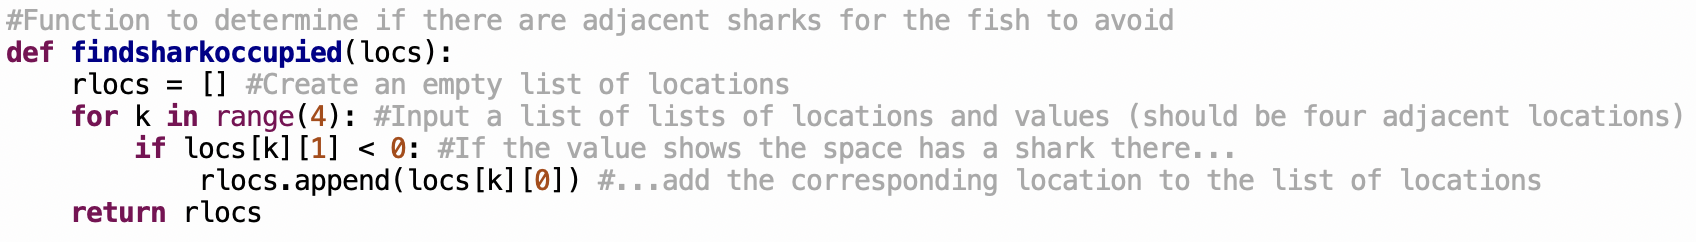
\includegraphics[width=0.95\textwidth]{findSharkOccupied.png}
  \caption{\label{fig:findSharkOccupied}
  Screenshot of the code for the function to find adjacent spaces occupied by sharks
  }
  \end{center}
\end{figure}


The next step was to actually use this function in the main function of the simulation to prevent the fish from being suicidal. 
The original code created two lists, oldlocs and newlocs, which check for adjacent empty spaces for the fish to move into using the removeoccupied function. 
It then found the intersection of these lists, placing it into a new list called availlocs. 
This new list held all of the empty adjacent spaces that the fish could move into, and if there were any available options, then the fish would choose one at random and move into it. 
In order to make our fish more realistic, however, we would need them to move into adjacent spaces that are empty but also not adjacent to a shark. 
Thus, we created four new lists: oldsharklocs, which scanned through the old array’s adjacent locations for sharks; newsharklocs, which scanned through the new array’s adjacent locations for sharks; sharklocs, which was the intersection of the former two lists; and actualavaillocs, the list of elements that were contained in availlocs but not in sharklocs. 
Instead of checking availlocs for available options to move into, the fish now checked actualavaillocs to satisfy the modification’s condition. 
Below is a screenshot of the modified code:


\begin{figure}[htbp]
  \begin{center}
  \item[]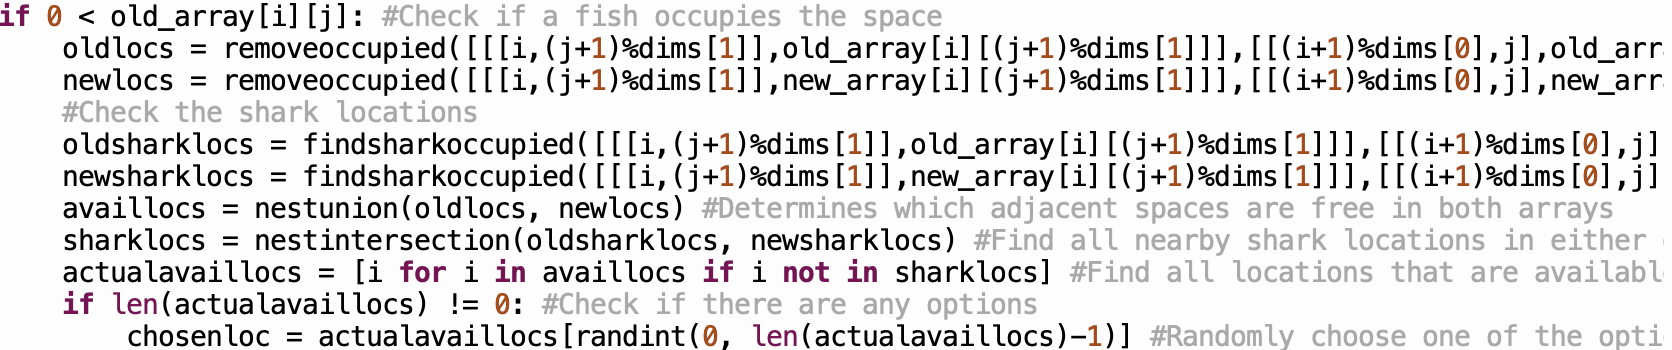
\includegraphics[width=0.95\textwidth]{modifiedFishMovement.png}
  \caption{\label{fig:modifiedFishMovement}
  Screenshot of the code used to modify the fish’s movement
  }
  \end{center}
\end{figure}


After running the simulation a few times with the rest of the parameters set to their defaults, some distinct trends were observed that differentiated this version from the original. 
In every run, the population of fish is much higher than that of the sharks, and the rises and drops in the graphs are not as dramatic as the original runs. 
These changes in population are also less periodic and seem more sporadic. 
This could be explained by the fact that the fish were less likely to be eaten at each step now, so they could maintain a more steady population with less sudden changes. 
In each of the runs, there was also an initial drop in population for both the fish and sharks, but then the fish would rise in population while the sharks would remain at a much lower population. 
This may be a result of the random initial distribution of the fish and shark populations – after “settling down”, the fish are able to repopulate and evade the sharks better while the sharks have a harder time catching up to them.

This modified simulation still bears some similarities to the original one, though. 
The populations do not remain constant, and there is some up and down movement, albeit not as pronounced as the original. 
The graphs also show how the shark population still lags 90 degrees behind the fish population, which is expected considering the sharks still have to wait for the fish to move and reproduce first before they can move. 
Below are some plots which exhibit the aforementioned behaviors:


\begin{figure}[htbp]
  \begin{center}
  \item[]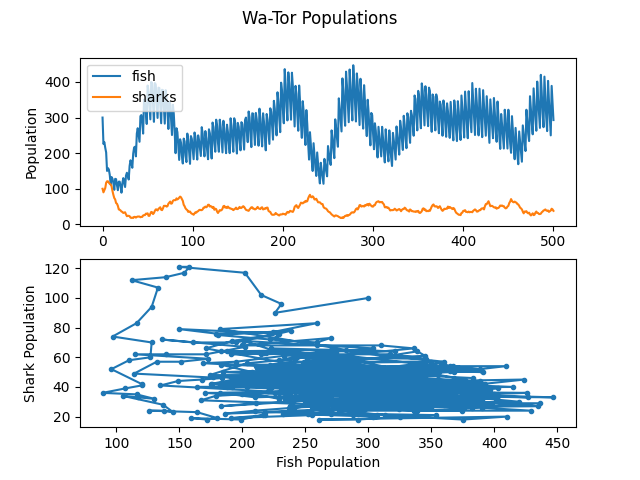
\includegraphics[width=0.75\textwidth]{run4plots.png}
  \end{center}
  \caption{\label{fig:run4plots}
  Modified Simulation Run 1
  }
\end{figure}

\begin{figure}[htbp]
  \begin{center}
  \item[]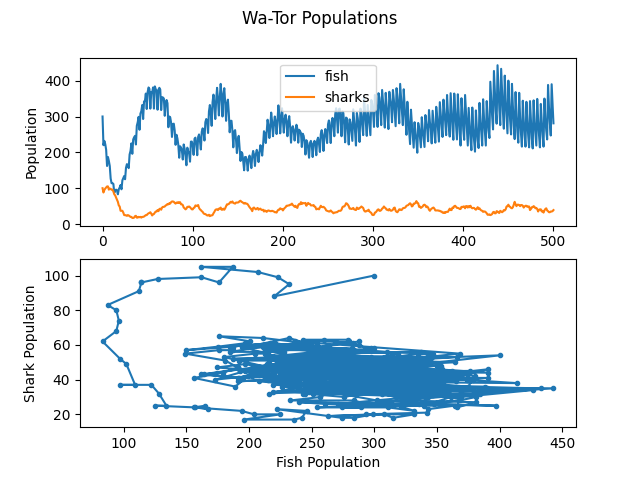
\includegraphics[width=0.75\textwidth]{run5plots.png}
  \end{center}
  \caption{\label{fig:run5plots}
  Modified Simulation Run 2
  }
\end{figure}

\begin{figure}[htbp]
  \begin{center}
  \item[]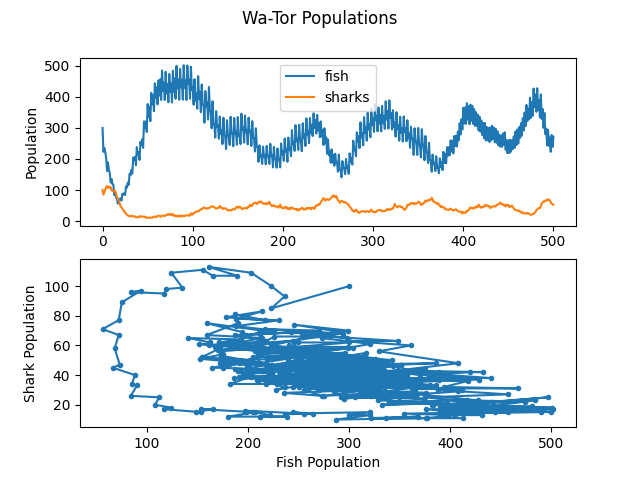
\includegraphics[width=0.75\textwidth]{run6plots.png}
  \end{center}
  \caption{\label{fig:run6plots}
  Modified Simulation Run 3
  }
\end{figure}

\end{document}
%%%%%%%%%%%%%%%%%%%% Document Ends %%%%%%%%%%%%%%%%%%%%
